\chapter{Elements of Room Acoustics}\label{chap:acoustics}
\vspace{-2.5em}
\newthought{Synopsis}
% \marginpar{%
%     \centering
%     \footnotesize
%     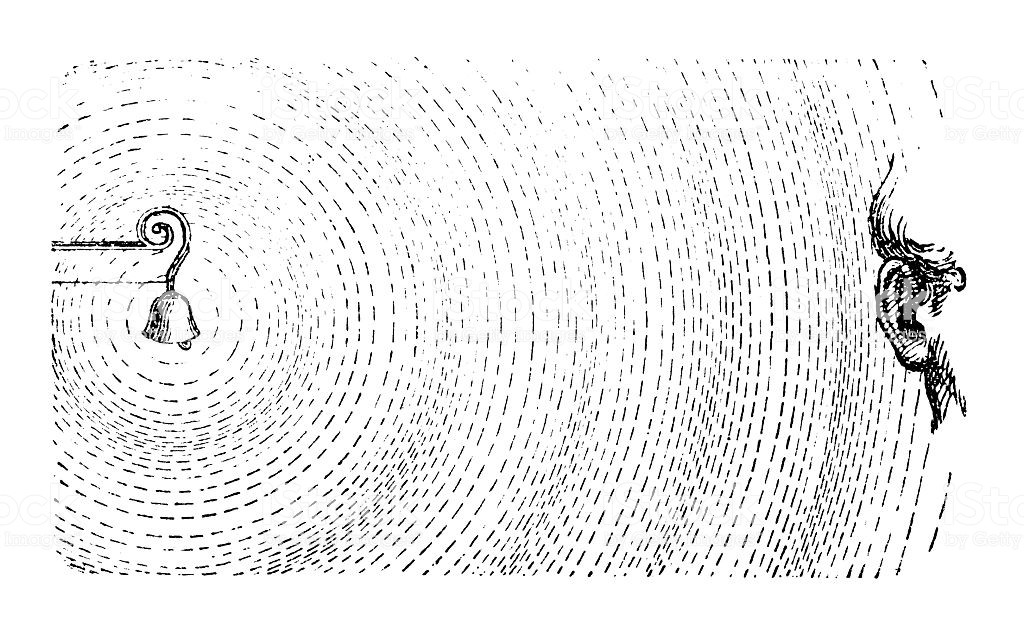
\includegraphics[width=\linewidth]{acoustics/sound_propagation.jpg}
%     \label{fig:acoustics:sound}
% }
\openepigraph{Sound, a certain movement of air.}{Aristotele, De Anima II.8 420b12}
This chapter will build a first important bridge: from acoustics to audio signal processing.
It first defines sound and how it propagates in the environment~\cref{ch:acoustics:sec:wave}, teasing out the fundamental concepts of this thesis: the echoes.~\cref{ch:acoustics:sec:reflection} and the \RIRdef/~\cref{ch:acoustics:sec:rir}.
By assuming some approximations, the \RIR/ will be described in all its parts in relation with methods to compute them.
Finally, in~\cref{ch:acoustics:sec:perception}, how the human auditory system perceives reverberation will be reported.
\\The material on waves and acoustic reflection is digested from classic texts on room acoustics and PDEs:
Kuttruff’s \textit{Room Acoustics}, Pierce's \textit{Acoustics: an introduction to its physical principles and applications}, Duffy’s \textit{Green’s Functions with Applications}.
Notions on acoustic simulators are extracted from the Habet's tutorial paper \textit{Room impulse response generator},
the \citeauthor{savioja2015overview}'s paper of geometrical acoustics, and the documentation of the acoustic simulator \textit{Wayverb} in~\citeonly{thomas2017wayverb}.
More technical details are reported in Appendix~\ref{ap:roomAcoustics}.

\section{Sound wave propagation}\label{ch:acoustics:sec:wave}%\marginpar{\footnotesize Namely, there is no sound in outer space.}
\marginpar{%
    \centering
    \footnotesize
    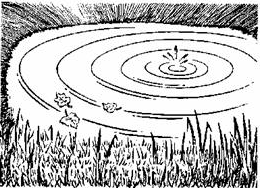
\includegraphics[width=\linewidth]{acoustics/lake.png}
    \captionsetup{labelformat=empty}
    \captionof{figure}{%
    Imagine a calm pond. The surface is flat and smooth. Drop a rock into it. \textit{Kerploop!} The surface is now disturbed.
    The disturbances spread propagate, as waves. The medium here is the water surface.
    }
    \label{fig:acoustics:lake}
}
According to common dictionaries and encyclopedias,
\begin{center}
    \textit{sound is the sensation perceived by the ear caused by the vibration of air}.
\end{center}
This definition highlights two aspects of sound: a physical one, characterized by the air particles vibration; and a perceptual one, involving the auditory system.
Focusing on the former phenomenon, when vibrating objects excites air, surrounding air molecules starts oscillating,
producing zones with different air densities leading to a compressions-rarefactions phenomenon.
Such vibration of molecules takes place in the direction of the excitement, with the next layer of molecules excited by the previous one.
Pushing layer by layer forward, a \textit{longitudinal mechanical wave}\sidenote{%
    As opposed to mechanical vibrations in a string or (drum) membrane,
    acoustic vibrations are \textit{longitudinal} rather than \textit{transversal},
    \ie/ the air particles are displaced in the same direction of the wave propagation.
} is generated.
Notice that therefore sound needs a medium to travel: it cannot travel through a vacuum and no sound is present in outer space.

Thus sound propagates though a medium, which can be solid, liquid or gaseous.
The propagation happens at a certain speed which depends on the physical properties of the medium, such as its density.
The medium assumed throughout the entire thesis is air, although extensions of the developed methods to other media could be envisioned.
Under the fair assumption of air being homogeneous and steady, the speed of sound can be approximated as follows:
\begin{equation}
    \cair =  331.4 + 0.6\temperature + 0.0124\rhumidity \hspace{1em} [\sfrac{\si{\metre}}{\si{\second}}]
    ,
\end{equation}
where $\temperature$ is the air temperature $[\si{\celsius}]$ and $\rhumidity$ is the relative air humidity $[\%]$.

The air pressure variations at one point in space can be represented by a \textit{waveform}, which is a graphical representation of a sound
~\cref{fig:acoustics:acoustics_wave}.
\begin{figure}[h]
    \centering
    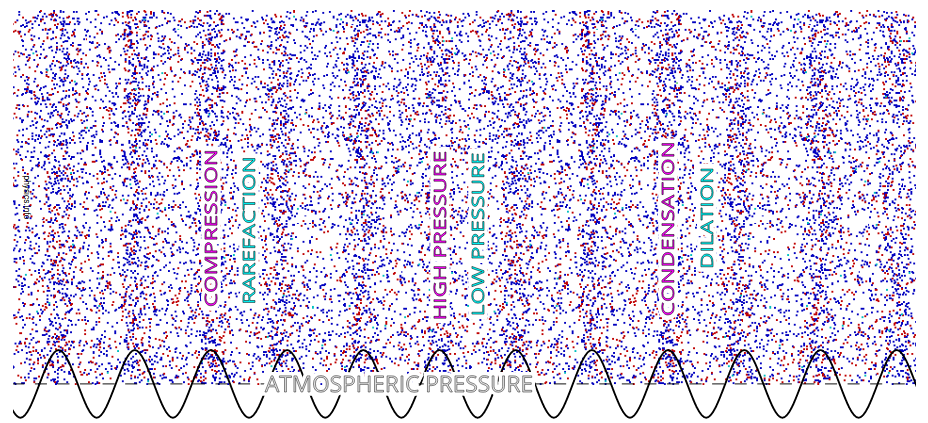
\includegraphics[width=\linewidth]{acoustics/acoustic_wave.png}
    \caption{snapshot of a longitudinal wave in air}
    \label{fig:acoustics:acoustics_wave}
\end{figure}

We can think of this process in the light of the classic \textit{source-medium-receiver} model of communication theory:
the \textit{source} is anything that emits waves\sidenote{%
    example of sources are vibrating solids (\eg/ loudspeakers membrane),
    rapid compression or expansion (\eg/ explosions or implosions)
    or air vortices with characteristics frequencies (\eg/ flute and whistles).
}, the \textit{medium} carries the waves from one point to another, and the \textit{receiver} absorbs them.

\subsection{The acoustic wave equation}\label{subsec:acoustics:waveq}
The acoustic wave equation is a second-order partial differential equation\sidenote{%
    In 1746, d’Alembert discovered the one-dimensional wave equation for music strings,
    and within ten years Euler discovered the three-dimensional wave equation for fluids.
} which describes the evolution of acoustic pressure $\pressure$
as a function of the position $\positionMicrophone$ and time $t$
\begin{equation}
    \label{eq:acoustics:wave}
    \knabla^2 \pressureSpaceTime - \frac{1}{\speedOfSound^2} \kpderiv[2]{\pressureSpaceTime}{t} = 0
    ,
\end{equation}
where $\knabla^2 = \kpderiv[2]{}{x} + \kpderiv[2]{}{y} + \kpderiv[2]{}{z}$ stands for the 3-dimensional \textit{Laplacian} operator.
The constant $\speedOfSound$ is the sound velocity in the medium and has dimension $\kbracket{\frac{\si{\metre}}{\si{\second}}}$.
\\Despite its complicated formulation, the wave equation is linear. Thus it implies the followings:
\begin{itemize}
    \item the pressure field at any time is the sum of the pressure fields resulting from each source at that time;
    \item the pressure field emitted at a given position propagates over space and time according to a linear operation.
\end{itemize}

\mynewline
Assuming the propagation of the wave in a homogeneous medium, one can obtain the equation above by combining three fundamental physical laws:
\begin{itemize}
    \item the \textit{conservation of momentum},
    \item the \textit{conservation of mass}, and
    \item the \textit{polytropic process relation}, meaning that the medium is an ideal gas undergoing a reversible adiabatic process.
\end{itemize}

However, media are not uniform and feature inhomogeneities of two types:
scalar inhomogeneities, \eg/ due to temperature variation,
and vector inhomogeneities, \eg/ due to presence of fans or air conditioning.
Although these affect the underlying assumption of the model, the effects are small in typical application of speech and audio signal processing.
Therefore they are commonly ignored.

\newthoughtpar{The Helmholtz's equation}
The equation~\ref{eq:acoustics:wave} is expressed in the space-time domain $\depSpaceTime$.
By applying the temporal Fourier transform, we obtain the \textit{Helmholtz equation}:
\begin{equation}
    \label{eq:acoustics:helmholtz}
    \knabla^2 P(\positionMicrophone, f) + k^2 P(\positionMicrophone, f) = 0
    ,
\end{equation}
where $k = \frac{2 \pi f}{c}$  is known as \textit{wave number} and relates the frequency $f$ to the propagation velocity $c$.

Both the wave~\ref{eq:acoustics:wave} and the Helmholtz's equation~\ref{eq:acoustics:helmholtz} are source-independent,
namely no source is present in the medium.
Therefore they are said to be \textit{homogeneous} as the right-hand term is zero.
Normally the sound field is a complex field generated by acoustics sources.
As consequence, the two equations become inhomogeneous as some non-zero terms needs to be added to the right-hand sides.

In the presence of a sound source producing waves with source function $s(t, \positionMicrophone)$, the wave equation can be written
\begin{equation}
    \label{eq:acoustics:source}
    \knabla^2 \pressureSpaceTime - \frac{1}{\speedOfSound^2} \kpderiv[2]{\pressureSpaceTime}{t} = s(t, \positionMicrophone)
    .
\end{equation}
Thus, the corresponding Helmholtz's equation writes
\begin{equation}
    \label{eq:acoustics:source_freq}
    \knabla^2 P(\positionMicrophone, f) - k^2 P(\positionMicrophone, f) = S(\positionMicrophone, f)
    .
\end{equation}

For instance one can assume an infinitesimally small pulsating sphere locate at $\positionSource$ radiating constant acoustic energy at frequency $f$,
\ie/ $S(\positionMicrophone) = \delta(\positionMicrophone - \positionSource)$.
At the receiver position $\positionMicrophone \neq \positionSource$, the Helmholtz's equation writes
\begin{equation}
    \label{eq:acoustics:green_definition}
    \knabla^2 H(f, \positionMicrophone \mid \positionSource)
        - k^2 H(f, \positionMicrophone \mid \positionSource)
        = \delta(\positionMicrophone - \positionSource)
    ,
\end{equation}
The function $H(f, \positionMicrophone \mid \positionSource)$ satisfying \cref{eq:acoustics:green_definition} is called the \textit{Green's function} and is
associated to ~\cref{eq:acoustics:helmholtz}, for which it is also a solution.
% \\In the next subsection, we will see that the function $H$ can be interpreted as the free-field \textit{Transfer Function}
% between the source at $\positionSource$ and the receiver at $\positionMicrophone$.

\subsection{... and its Green solution}
\marginpar{%
    \footnotesize
    By 1950 Green’s functions for Helmholtz’s equation were used to find the
    wave motions due to flow over a mountain  and in acoustics.
    Green’s functions for the wave equation lies with Gustav Robert Kirchhoff (1824–1887),
    who used it during his study of the three-dimensional wave equation.
    He used this solution to derive his famous \textit{Kirchhoff’s theorem}~\citeonly{duffy2015green}.
}
Green's Functions are mathematical tools for solving linear differential equations with specified initial- and boundary- conditions~\citeonly{duffy2015green}.
They have been used to solve many fundamental equations, among which \cref{eq:acoustics:helmholtz,eq:acoustics:wave} for both free and bounded propagation.
They can be seen as a concept analogous to \emph{impulse responses}\sidenote{Impulse responses in time domain, transfer functions in the frequency domain.} in signal processing.
Under this light, the physic so-far can be rewritten using the vocabulary of the communication theory, namely \textit{input}, \textit{filter} and \textit{output}.

According to Green's method, the equations above can be solved in the frequency domain for arbitrary source as follows:
\begin{equation}
    \label{eq:acoustics:helmholz_conv}
    P(f, \positionMicrophone) = \iiint_{\volume_\contSource} H(f, \positionMicrophone \mid \positionSource) S(f, \positionSource) \kdiff\positionSource
    ,
\end{equation}
where $\volume_\contSource$ denotes the source volume,
and  $\kdiff\positionSource =  \kdiff{x_\contSource}\,\kdiff{y_\contSource}\,\kdiff{z_\contSource}$ the  differential  volume element at position $\positionSource$.
If one ignores the space integral, one can see the close relation with a transfer function.
\\The requested sound pressure $\pressureSpaceTime$ can now be computed by taking the frequency-directional inverse Fourier transform of \cref{eq:acoustics:helmholz_conv}.

It can be shown \citeonly{kuttruff2016room} that the Green's function for~\cref{eq:acoustics:helmholtz,eq:acoustics:green_definition} writes
\begin{equation}
    \label{eq:acoustics:greenFreeFreq}
    H(f, \positionMicrophone \mid \positionSource) = \frac{1}{4 \pi \norm{\positionMicrophone - \positionSource}} \cste^{- \frac{\csti 2 \pi f \norm{\positionMicrophone - \positionSource}}{\speedOfSound}}
\end{equation}
where $\norm{\cdot}$ denotes the Euclidean norm.
\marginpar{
    \footnotesize
    \cref{eq:acoustics:greenFreeFreq,eq:acoustics:greenFreeTime} are respectively the free-field transfer function and the impulse response.
}
By applying the inverse Fourier transform to the result above, we can write the time-domain Green's function as
\begin{equation}
    \label{eq:acoustics:greenFreeTime}
    h(t, \positionMicrophone \mid \positionSource) =
        \frac{1}{4 \pi \norm{\positionMicrophone - \positionSource}}
        \diracOf{t - \frac{\norm{\positionMicrophone - \positionSource}}{\speedOfSound}}
\end{equation}
where $\diracOf{\cdot}$ is the time-directional Dirac delta function.
\\As consequence, the \textit{free field}, that is open air without any obstacle, the  sound propagation incurs a delay $\distMicSrc / c$
and an attention $1 / (4 \pi \distMicSrc)$ as function of the distance
$ \distMicSrc = \norm{\positionMicrophone - \positionSource}$ from the source to the microphone.

According to \cref{eq:acoustics:greenFreeTime}, the sound propagates away from a point source with a spherical pattern.
When the receiver is far enough from the source, the curvature of the \textit{wavefront} may be ignored.
The waves can be approximated as \textit{plane waves} orthogonal to the propagation direction.
This scenario depicted in \cref{fig:acoustics:planewaves} is known as \textit{far-field}.
\marginpar{%
    \centering
    \footnotesize
    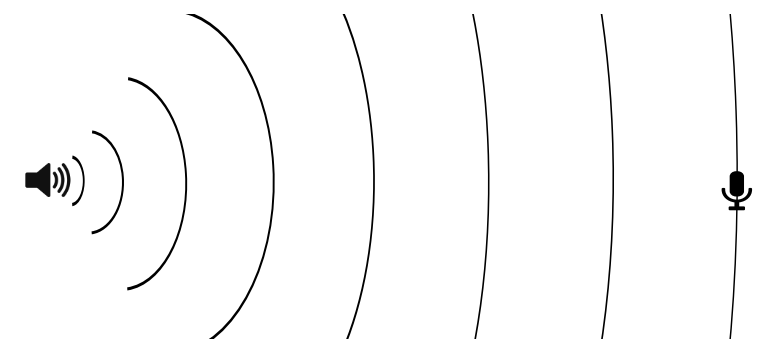
\includegraphics[width=\linewidth]{acoustics/planewaves.png}
    \captionof{figure}{%
    Visualization of the sound propagation. Since the sensor (i.e. a microphone)
    is drawn in the far field, the incoming waves can be approximated as plane waves.
    }
    \label{fig:acoustics:planewaves}
}
In contrast, when the distance between the source and the receiver is small, the scenario is called \textit{near field}.

%%%%%%%%%%%%%%%%%%%%%%%%%%%%%%%%%%%%%%%%%%%%
\section{Acoustic reflections}\label{ch:acoustics:sec:reflection}
The equations derived so far assumed unbounded medium, \ie/ free space: a rare scenario in everyday applications.
Real mediums are typically bounded, at least partially.
For instance in a room, the air (propagation medium) is bounded by walls, ceiling, and floor.
When sound travels outdoor, the ground acts as a boundary for one of the propagation directions.
Therefore, the sound wave does not just stop when it reaches the end of the medium or when it encounters an obstacle in its path.
Rather, a sound wave will undergo certain behaviors depending on the obstacles' acoustics and geometrical properties, including
\begin{itemize}
    \item \textit{reflection} off the obstacle,
    \item \textit{diffraction} around the obstacle, and
    \item \textit{transmission} into the obstacle, causing
    \begin{itemize}
        \item \textit{refraction} through it, and
        \item \textit{dissipation} of the energy.
    \end{itemize}
\end{itemize}
\marginpar{%
    \centering
    \footnotesize
    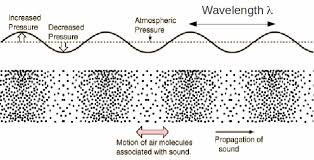
\includegraphics[width=\linewidth]{acoustics/wavelength.jpg}
    \captionof{figure}{%
        wavelength
    }
    \label{fig:acoustics:wavelength}
}

\newthought{Reflections typically arise} when a sound wave hits a large surface, like a room wall.
When the sound meets a wall edge or a slit, the wave diffracts, namely it bends around the corners of an obstacle.
The point of diffraction effectively becomes a secondary source which may interact with the first one.
\\The part of energy transmitted to the object may be absorbed and refracted.
Objects are characterized by a proper acoustic resistance, called \textit{acoustic impedance}, which
describes their acoustic inertia as well as the energy dissipation.
The remaining contribution may continue to propagate resulting in the refraction phenomenon\sidenote{%
    This is more commonly observed when light passes thought different medium, like a prism.
}.

When sound reflects on an solid surface, two types of acoustic reflections can occur: part of the sound energy
\marginpar{%
    \centering
    \footnotesize
    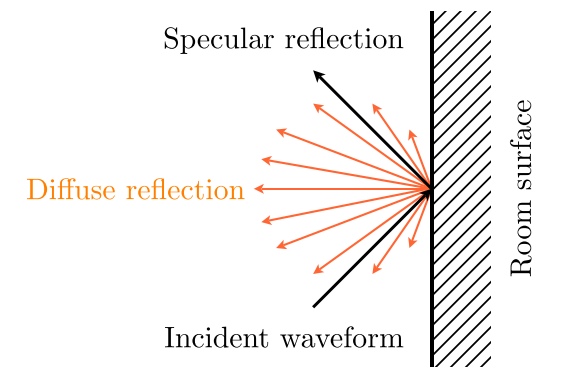
\includegraphics[width=\linewidth]{acoustics/reflection.png}
    \captionof{figure}{%
        Specular vs diffuse reflection
    }
    \label{fig:acoustics:reflection}
}
\begin{itemize}
    \item is reflected \textit{specularly}, \ie/, the angle of incidence equals the angle of reflection; and
    \item is reflected \textit{diffusely} - or \textit{scattered}, \ie/, scatter in every direction).
\end{itemize}

All the phenomena occur with different proportions depending on the acoustics and geometrical properties of surfaces and the frequency content of the wave.
In acoustics, it is common to define the \textit{operating points} and different \textit{regimes}\sidenote{for instance near- \vs/ far-field}
according to the sound frequencies or the corresponding \textit{wavelength},
\begin{equation}
    \wavelength = \frac{2 \pi}{k} = \frac{\speedOfSound}{f} \mathspace [\si{\metre}]
    ,
\end{equation}
where $f$ is the frequency of the sound wave.

\openepigraph{
    Sabine had previously used ray-based acoustics in the
    early 1900s to investigate sound propagation paths using Schlieren photography.
    Their impressive visualizations show wavefronts that are augmented
    with rays that are perpendicular to the wavefronts.}{\citeonly{savioja2015overview}}

As depicted in~\cref{fig:acoustics:wavelength}, $\wavelength$ measures the spatial distance between two points around which the medium has the same value of pressure.
% \marginpar{%
%     \footnotesize
%     a frequency of $\SI{1}{\kHz}$ corresponds to a wavelength of approximately $\SI{34}{\cm}$ ,
%     which is one or two orders of magnitude smaller than typical linear dimensions of rooms,
%     as well as typical distances traveled by sound waves in a room
% }.
\marginpar{
    \centering
    \footnotesize
    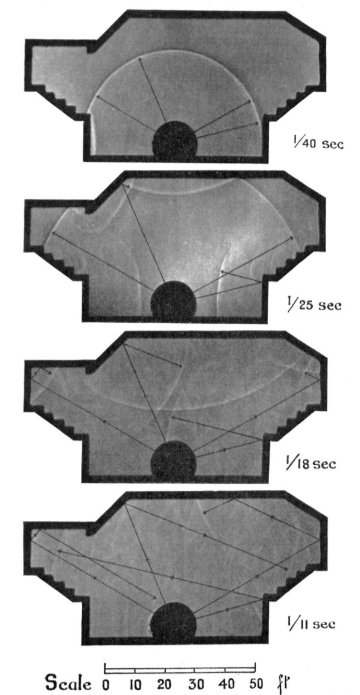
\includegraphics[trim={0 205 0 0},clip,width=\linewidth]{acoustics/sound_pulse1926.png}
    \captionsetup{labelformat=empty}
    \captionof{figure}{%
        Photographs showing successive stages in the progress of a sound pulse in a section of a Debating Chamber.
        \imgsrc{\citeonly{davis1926sound}}
    }
    \label{fig:acoustics:reflection}
}
\\Using this quantity we can identify the following three responses of objects (irregularities) of size $d$ to a plane-wave, as depicted in~\cref{fig:acoustics:irregularities}
\begin{figure}
    \footnotesize
    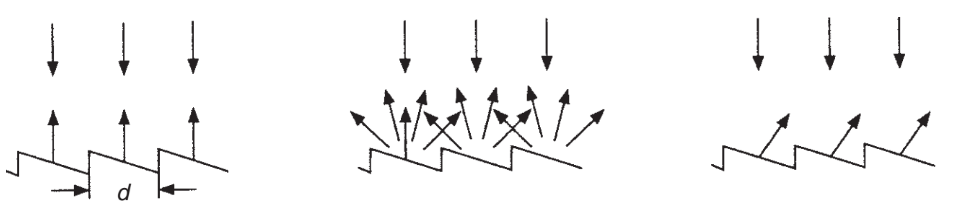
\includegraphics[width=\linewidth]{acoustics/irregularities.png}
    \captionof{figure}{%
        A reflector having irregularities on its surface with width $d$ much smaller than the sound wavelength $\wavelength$.
        Image courtesy of \citeonly{kuttruff2016room}.
    }
    \label{fig:acoustics:irregularities}
\end{figure}
\begin{itemize}
    \item $\wavelength \gg d$, the irregularities are negligible and the sound wave reflection is of specular type;
    \item $\wavelength \approx d$, the irregularities break the sound wave which is reflected towards every direction;
    \item $\wavelength \ll d$, each irregularities is a surface reflecting specularly the sound waves.
\end{itemize}

\mynewline
This presented behavior can be described with the wave equation by imposing adequate boundary conditions.
% However working with this formula might results complicated and difficult.
A simplified yet effective approach - just as in optics - is to model incoming sound waves as \textit{acoustic rays}~\citeonly{davis1926sound, krokstad1968calculating}.
A ray has well-defined direction and velocity of propagation, and conveys a total wave energy which remains constant.
This simplified description undergoes with the name of \GAdef/~\citeonly{savioja2015overview}, and share many fundamentals with geometrical optics.
This model will be convenient to describe and visualize the reflection behavior hereafter.

\subsection{Large smooth surfaces, absorption and echoes}
% The main focus of this section and the this whole thesis goes on \textit{specular reflections}.
Specular reflections are generated by surfaces which can be modelled as infinite, flat, smooth and rigid.
As mentioned above, this assumption is valid as long as the surface has dimension much larger than the sound wavelength.
Here the acoustic ray is reflected according to the \textit{law of reflection}, stating that
(i) the reflected ray remains in the plane identified by the incident ray and the normal to the surface,
and (ii) the angles of the incident and reflected rays with the normal are equal.
\marginpar{%
    \centering
    \footnotesize
    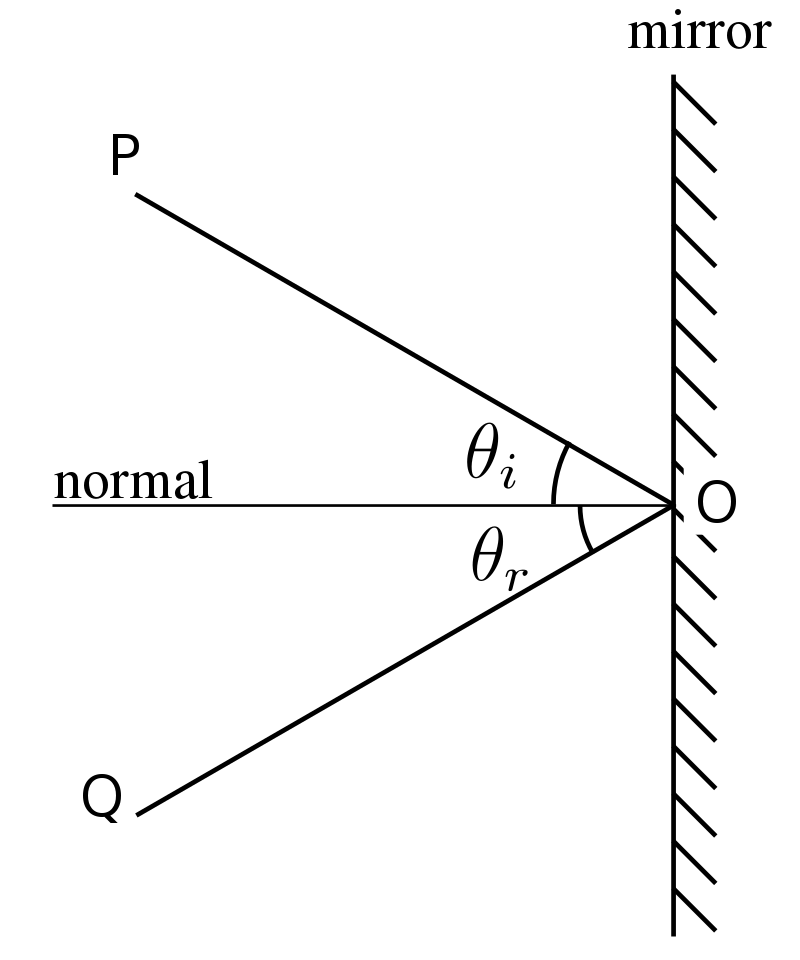
\includegraphics[width=\linewidth]{acoustics/reflection_law.png}
    \captionof{figure}{%
        Schematic representation of specular reflection.
    }
    \label{fig:acoustics:reflection_law}
}

If the surface $\surface$ is not perfectly rigid or impenetrable, its behavior is described by the \textit{acoustic impedance}, $\impedence_\surface(f) \in \bbC$.
%\sidenote{\textbf{acoustic impendence} measures the opposition that an acoustic system presents to the acoustic pressure}.
Analytically, it is defined as a relation between sound pressure and particle velocity at the boundary.
It consists of a real and imaginary part, called respectively acoustic \textit{resistance} and \textit{reactance}.
The former can be seen as the part of the energy which is lost, and the latter as the part which is stored.

\newthought{The reflection coefficient} $\reflCoeff$ can be derived from the acoustic impedance
for plane waves, \ie/ under assuming a far-field regime between source, receiver and surface.
\begin{quote}
    \textit{It measures the portion of energy absorbed by the surface
    \\and the incident acoustic wave.}
\end{quote}
Analytically, it is defined as  \citeonly{kuttruff2016room,pierce2019acoustics}
\begin{equation}
    \reflCoeff(f, \theta) = \frac{\impedence_\surface(f)\cos{\theta} - \impedenceAir(f)}{\impedence_\surface(f)\cos{\theta} + \impedenceAir(f)}
    ,
\end{equation}
where $\impedence_\surface(f)$ and $\impedenceAir(f)$ are the frequency-dependent impedance of the surface and the air respectively,
and $\theta$ is the angle of incidence.

\newthought{The absorption coefficient} is typically used instead in the context of \GA/ and audio signal processing.
It comes from the following approximations~\citeonly{savioja2015overview}:
(\textit{i}) the energy or intensity of the plane wave\sidenote{%
    Since it is the square magnitude of the acoustic pressure, the phase information is lost.
}, is considered instead of the acoustic pressure;
(\textit{ii}) dependency on the angle of incidence is relaxed in favor of the averaged quantities;
(\textit{iii}) local dependency on frequencies is relaxed in favor of a frequency-independent scalar or at most a description per octave-band.
These assumptions are motivated by the difficulty of measuring the acoustic impedance
and the possibility to compute an equivalent coefficient a posteriori

Therefore, it is customary to use the absorption coefficient, defined as
\begin{equation}
    \absCoeff(f) = 1 - \abs{\bar{\reflCoeff}(f)}^2
    ,
\end{equation}
where $\bar{\reflCoeff}$ is the reflection coefficient averaged over the angles $\theta$.

\newthought{Echoes are specular reflections}\marginpar{%
    \footnotesize
    The word echo derives from the Greek \textit{echos}, literally ``sound''.
    In the folk story of Greek, Echo is a mountain nymph whose ability to speak was cursed:
    she only able to repeat the last words anyone spoke to her.
} which stand out in terms of energy strength or timing.
Originally this term is used to refer to sound reflections which are subjectively noticeable as a separated repetition of the original sound signal.
These can be heard consciously in outdoor scenario, such as in mountain. However, they are less noticeable to the listener in close rooms.
In~\cref{ch:acoustics:subsec:rir} a proper definition of echoes will be given with respect to the temporal distribution of the acoustic reflections.

\subsection{Diffusion, scattering and diffraction of sound}
Real-world surfaces are not ideally flat and smooth; they are rough and uneven.
Examples of such surfaces are coffered ceilings, faceted walls, raw brick walls as well as the entire audience area of a concert hall.
When such irregularities are in the same order as the sound wavelength, \textit{diffuse reflections} is observed.

In the context of \GA/, the acoustic ray associated to a plane-wave can be though of as a bundle of rays traveling in parallel.
When it strikes such a surface, each individual rays are bounced off irregularly, creating \textit{scattering}:
a number of new rays are created, uniformly distributed in the original half-space.
The energy carried by each of the outgoing ray is angle dependent and it
is well modeled thought the \textit{Lambert's cosine law}, originally used to describe optical diffuse reflection.

The total amount of energy of this reflection may be computed a-priori
knowing the \textit{scattering} coefficient of the surface material.
Alternatively, it can be derived a-posteriori with the \textit{diffusion coefficient}, namely the ratio between
the specularly reflected energy over the total reflected energy.

\textit{Diffraction waves} occur when the sound confronts the edge of a finite surface, for instance around corners or through door openings.
This effect is shown in~\cref{fig:acoustics:diffraction}
\marginpar{%
    \centering
    \footnotesize
    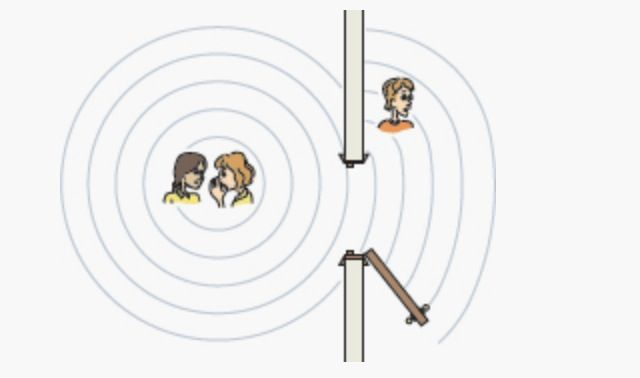
\includegraphics[width=\linewidth]{acoustics/sound_diffraction.jpg}
    \captionof{figure}{%
        Schematic representation of sound diffraction.
        This effect allows to hear ``behind walls''.
    }
    \label{fig:acoustics:diffraction}
}
At first the sound wave propagates spherically from the source.
Once it reaches the reflector's  apertures, the wave is diffracted, \ie/ bended, behind it.
It is interesting to note that the diffraction waves produced by the semi-infinite reflector edge
allow the area that is ``behind'' the reflector to be reached by the propagating sound.
This physical effect is exploited naturally by the human auditory system to localize sound sources.

% -----------------------------------------------------------------------------
\section{Room acoustics and room impulse response}\label{ch:acoustics:sec:rir}
Room acoustics is concerned with acoustic waves propagating in air enclosed in a volumes with a set of surfaces
(walls, floors, etc.), which an incident wave may be interacts with as described in \cref{ch:acoustics:sec:reflection}.
In this context, a
\begin{center}
    \textit{A room is a physical enclosure containing the medium and with boundaries limiting the sound propagation.}
\end{center}

Mathematically, the sound propagation is described by the wave equation~\eqref{eq:acoustics:wave}.
By solving it, the \AIRdef/\sidenote{The \ATFdef/ is the Fourier transform of the \AIR/}
from a source to a microphone can be obtained.
In the context of room acoustics, it is commonly referred to as the \RIRdef/, usually stressing
the geometric relation between reflections and the geometry of the scene.
In this thesis the two terms will be used indistinctly.

\subsection{The room impulse response}\label{ch:acoustics:subsec:rir}
The \RIRdef/ is where physical room acoustic and indoor audio signal processing meets and from now on, we will adopt a signal processing perspective.
Therefore
\begin{center}
\textit{the \RIR/ as a causal time-domain filter that accounts for the whole indoor sound propagation
from a source to a receiver}
\end{center}
\cref{fig:acoustics:rir} provides a schematic illustration of the shape of a \RIR/ compared to a measured one.
\begin{figure}[h]
    \centering
    \begin{minipage}[b]{.5\textwidth}
        \centering
        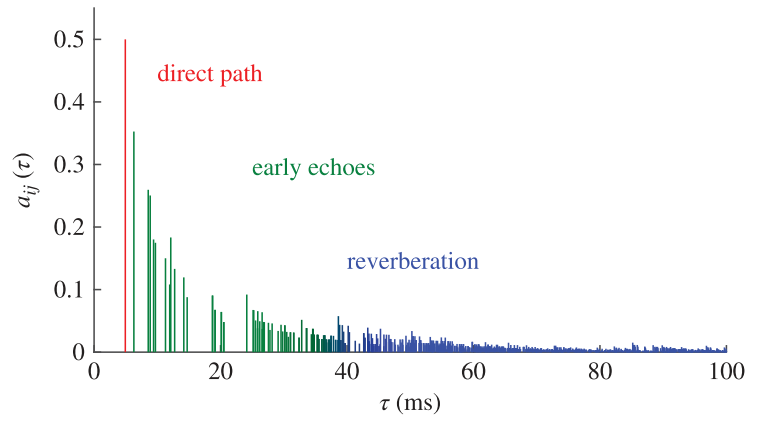
\includegraphics[width=\linewidth]{acoustics/rir_schematic.png}
    \end{minipage}%
    \begin{minipage}[b]{.5\textwidth}
        \centering
        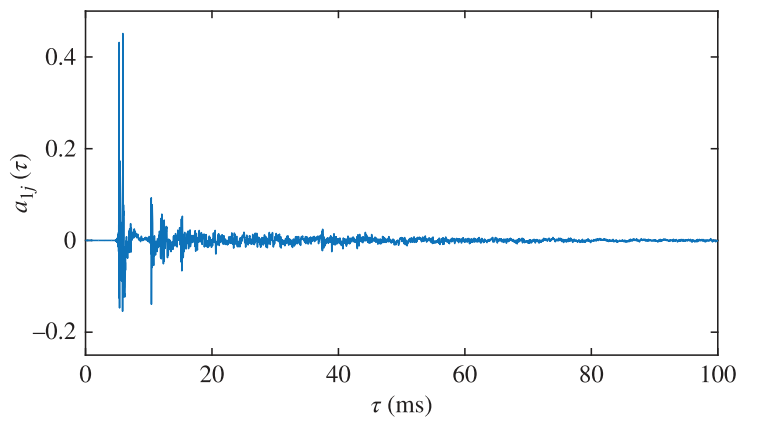
\includegraphics[width=\linewidth]{acoustics/rir_measured.png}
    \end{minipage}
    \caption{Schematic illustration of the shape of an \RIR/ and the first 100 ms of a measured one.}
    \label{fig:acoustics:rir}
\end{figure}

The \RIRs/ usually exhibit common structures.
Based on the consideration of~\cref{ch:acoustics:sec:reflection}, they are commonly divided into three partially overlapped components:
\begin{equation}\label{eq:acoustics:rir_full}
\rir(t) = h^d(t) + h^e(t) + h^l(t)
,
\end{equation}

where
\begin{description}
    \item[the direct path] $h^d(t)$ is the line-of-sight contribution of the sound wave.
    This term coincides with the ``pure delay'' modeled by the free-field propagation model~\eqref{eq:acoustics:greenFreeTime}.
    \item[the acoustics echoes or early refelctions] are included in $h^e(t)$ comprising few disjoint reflections coming typically from room surfaces.
    They are usually characterized by sparsity in the time domain and greater prominence in amplitude.
    These first reflections are typically specular and are well modeled in general by the \ISMdef/ explained in \cref{subsec:acoustics:ism}.
    \item[the late reverberation], or simply \textit{reverberation}, $h^l(t)$ collects many reflections occurring simultaneously.
    This part is characterized by a diffuse sound filed with exponentially decreasing energy.
\end{description}
These three components are not only ``visible'' when plotting the \RIR/ against time,
but they are characterized by different perceptual features, as explained~\cref{ch:acoustics:sec:perception}.

% IDEAL \vs/ MULTIPATH \vs/ REVERBERANT benesty
\mynewline
To conclude, let $s(t)$ be the source signal. The received sound writes
\begin{equation}
    x(t) = (\rir \convCont s)(t)
    ,
\end{equation}
where the symbol $\convCont$ is the continuos-time convolution operator.

Apart for certain simple scenarios, computing \RIRs/ in closed forms is a cumbersome task.
Therefore numerical solvers or approximate models are used instead.

\subsection{Simulating room acoustics}\label{sec:acoustics:simulators}
\marginpar{
    \footnotesize
    The docoumentation of the \href{https://reuk.github.io/wayverb/introduction.html}{Wayverb}
    acoustic simulator offers a complete overview of
    the \SOTA/ in acoustic simulator methods~\citeonly{thomas2017wayverb}.}
Most of the simulators available falls in three main categories:
\begin{description}
    \item[the wave-based simulators] aims at solving the wave equation numerically;
    \item[geometric simulators] make some simplifying assumption about the wave propagation.
    They typically ignore the wave physic, instead they adopt much lighter models such as \textit{ray}s or \textit{particle}s;
    \item[the hybrid simulators] combining both approaches.
\end{description}

\newthought{Wave-based Methods} are iterative methods that divide the 3D bounded enclosure into a grid of interconnected nodes
\sidenote{\ie/ mechanical unit with simple degrees of freedoms, like mass-spring system or one-sample-delay unit}.
For instance, the \FEM/ divides the space into small volume elements smaller than the sound wavelengths,
while the \BEM/ divides only the boundaries of the space into surface elements.
These nodes interact with each other according to the math of the wave equation.
Unfortunately, simulating higher frequencies requires denser interconnection-, so the computational complexity increases.
The \FDTDf/ method replaces the derivatives with their discrete approximation, \ie/ finite differences.
The space is divided into a regular grid, where the changes of a quantity (air pressure or velocity ) is computed over time at each grid point.
\DWMf/ methods are a subclass of \FDTD/ often used in acoustics problem.
\marginpar{
    \centering
    \footnotesize
    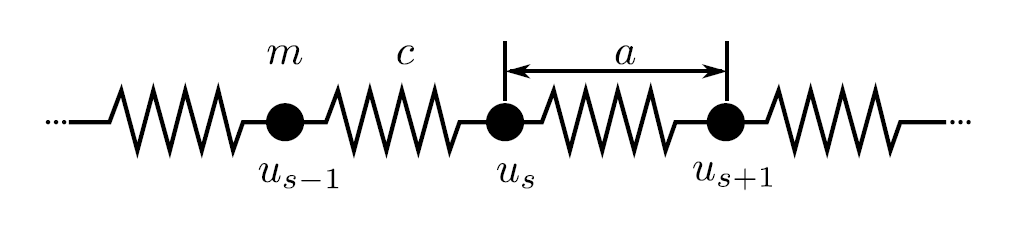
\includegraphics[width=\linewidth]{acoustics/mass_spring_model.png}
    \captionof{figure}{%
        Example of a mass-spring linear mesh used to simulate a 1D transversal wave.
    }
    \label{fig:acoustics:dwm}
}

\begin{figure}[t]
    \begin{fullwidthfig}
        \centering
        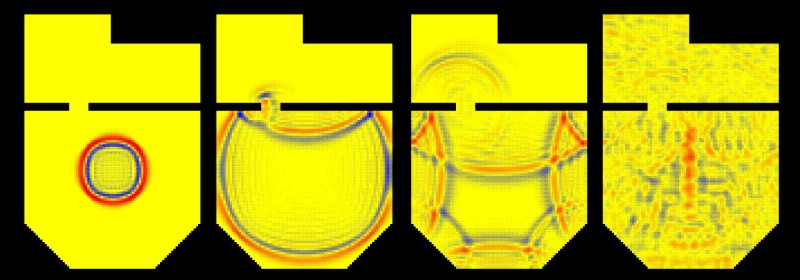
\includegraphics[width=\linewidth]{acoustics/simulator_dwg.jpg}

        \caption{Simulation of Sound propagation at four consecutive timestamps using the \DWM/ technique.
        A short, sharp, impulsive sound fired into the larger of two rooms causes a circular wavefront to spread out from the sound source.
        The the wave is reflected from the walls and part of it passes through a gap into the smaller room.
        In the larger room, interference effects are clearly visible;
        in the smaller room, the sound wave has spread out into an arc, demonstrating the effects of diffraction.
        A short while after the initial event, the sound energy has spread out in a much more random and complex fashion.
        }
        \label{fig:acoustics:dwm}
    \end{fullwidthfig}

\end{figure}

\begin{figure}[t]
    \begin{fullwidthfig}
        \label{fig:acoustics:fdtd}
        \centering
        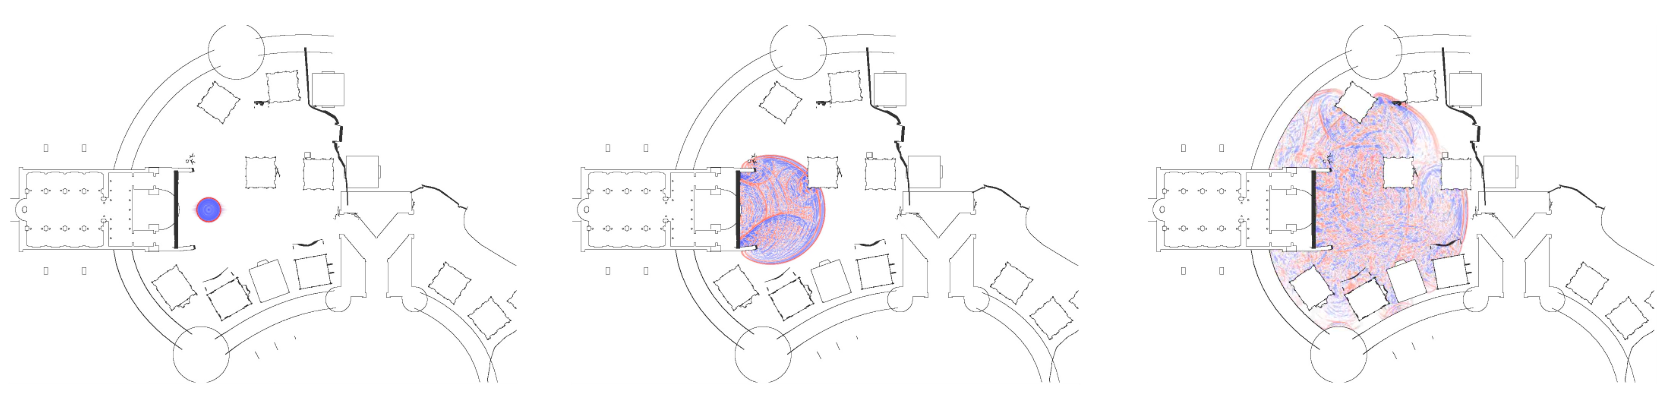
\includegraphics[width=\linewidth]{acoustics/wave-simulation_fdtd.png}
    \end{fullwidthfig}

    \vspace{-\baselineskip}\vspace{-\baselineskip}
    \sideparmargin{outer}
    \sidepar{\vspace{\baselineskip}
        \caption{Sound propagation at three consecutive timestamps using the \FDTD/-based \textit{Triton} simulator from Microsoft}
        \label{fig:acoustics:fdtd}
    }

\end{figure}

\mynewline
The main drawback of these methods is discretisation:
less dense grids may simplify too much the simulation, while denser grids increase the computational load.
Moreover, they require delicate definitions of the boundary condition at the physical level,
like knowing complex impedances, which are rarely available in practice.
On the other hand these methods inherently account for many effects such as occlusion, reflections, diffusion, diffractions and interferences.
In particular, by simulating accurately low-frequencies components of the \RIR/, they are able to well characterize the \textit{room modes}
\sidenote{
    Room modes have the effect of amplifying and attenuating specific frequencies in the \RIR/,
    and produce much of the subjective sonic ``colour'' of a room.
    Their analysis and synthesis is of vital importance for evaluating acoustic of rooms,
    such as concert hall and recording studios or when producing musically pleasing reverbs.
},
namely, collections of resonances that exist in a room and characterize it.
\\As stated in \citeonly{valimaki2016more}, among the wave-based methods, the \DWMs/ are usually preferred:
they run directly in the time domain, requiring typically an easier implementation, and they exhibit a high level of parallelism.

\newthought{Geometric metods}
\marginpar{
    \footnotesize
    For a detailed discussion about geometric acoustic methods, please refer to \citeonly{savioja2015overview}.
} can be sub-grouped into \textit{stochastic} and \textit{deterministic} approaches.
They typically compute the reflection path(s) between the source and the receivers,
assuming that the wave behaves like a particle or a ray carrying the acoustic energy around the scene.

\mynewline
\textsc{Stochastic methods} are approximate by nature.
They are based on statistical modeling of the \RIRs/ or Monte Carlo simulation methods.
The formers writes statistical signal processing models based on prior knowledge,
such as probability distribution of the \RIR/ in regions of the time-frequency domain~\citeonly{badeau2019common}.
Rather than the detailed room geometry, these methods generally use high-level descriptors\sidenote{such as the amount of reverberation or source-to-receiver distance.}
to synthesize \RIRs/ and in some application are preferable.
The latters randomly and repeatedly subsample the problem space, \eg/ tracing the path of random reflections,
recording samples which fulfil some correctness criteria, and discarding the rest.
By combining the results from multiple samples, the probability of an incorrect result is reduced, and the accuracy is increased.
Typically the trade-off between quality and speed of these approaches is based on the number of samples and
the quality of the prior knowledge modeled.

\marginpar{
    \centering
    \footnotesize
    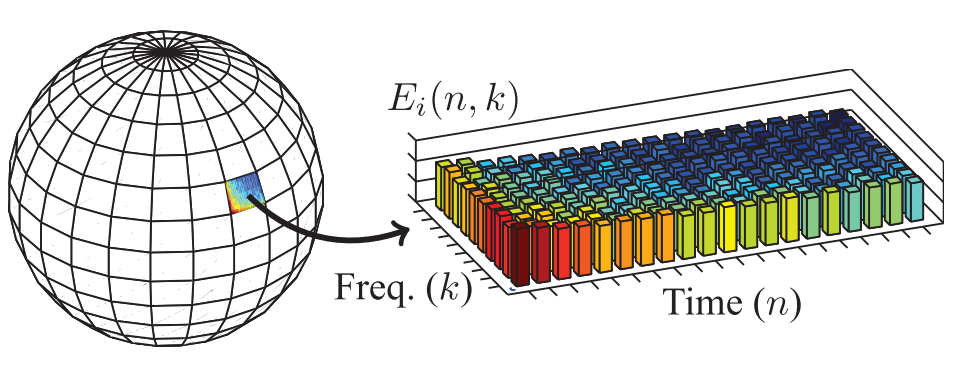
\includegraphics[width=\linewidth]{acoustics/simulator_diffuse_map.png}
    \captionof{figure}{%
        Directional-time-frequency Energy map resulting form the diffuse rain algorithm~\citeonly{schroder2007fast}.
        For each direction, that is receiver's spherical bin, a time-frequency histogram collects the energy of incoming rays.
        \imgsrc{\citeonly{schimmel2009fast}}
    }
    \label{fig:acoustics:diffuse_map}
}

\mynewline
\textit{Ray-tracing}~\citeonly{kulowski1985algorithmic} is one the most common methods that fall in this category and is very popular in the field of computer graphics for light simulation.
The basic idea is to collect ``valid'' paths of discrete rays traced around the room.
Many technique have been proposed to reduce the computational load, among which the \textit{diffuse rain algorithm}~\citeonly{schroder2007fast, heinz1993binaural} is commonly used in many acoustic simulators.
Each ray trajectory is reflected in a random direction every time it hits a wall and its energy is scaled according to the wall absorption.
The process of tracing a ray is continued until the ray’s energy falls below a predefined threshold.
At each reflection time and for each frequency (bin or band), the ray's energy and angle of arrival are recorded in histograms,
namely a \textit{directional-time-frequency energy map} of the room’s diffuse sound field for a given receiver location (\cfr{~\cref{fig:acoustics:diffuse_map}}).
This map is then used as prior distribution for drawing random sets of impulses which are used to form the \RIR/.
While lacking a detailed description of early reflections and room modes,
these methods are good to capture and simulate the statistical behavior of the diffuse sound field at a low computational cost.

\marginpar{
    \centering
    \footnotesize
    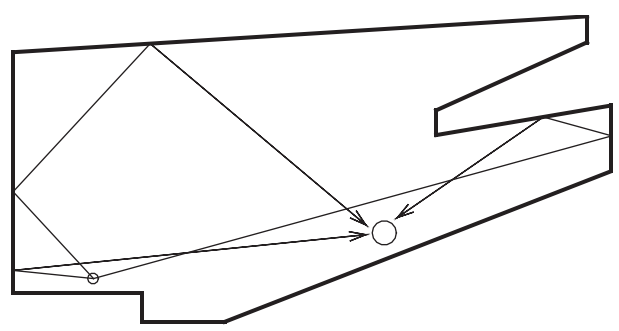
\includegraphics[width=\linewidth]{acoustics/simulator_ray1.png}
    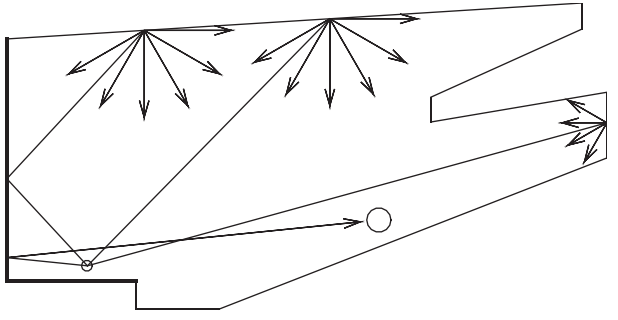
\includegraphics[width=\linewidth]{acoustics/simulator_ray2.png}
    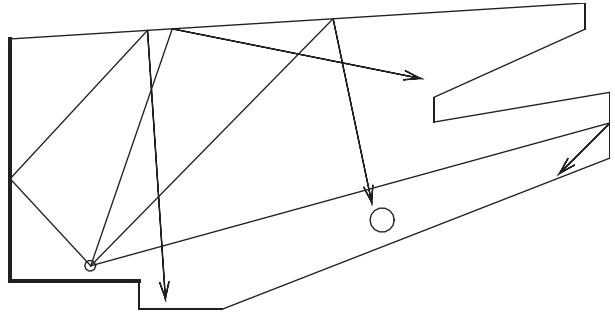
\includegraphics[width=\linewidth]{acoustics/simulator_ray3.png}
    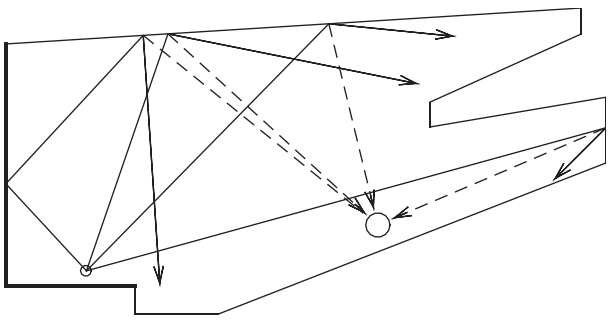
\includegraphics[width=\linewidth]{acoustics/simulator_ray4.png}
    \captionof{figure}{%
        Visualization of ray-tracing method.
        From top to bottom: first the method will eventually find specular reflection;
        then diffuse reflections can be modeled either by splitting a ray into several new rays or a single random one.
        In the diffuse rain technique a shadow-ray is cast from each diffuse reflection
        point to the receiver to speed-up convergence of the simulation.
        \imgsrc{\citeonly{savioja2015overview}}
    }
    \label{fig:acoustics:simulator_ray}
}

\mynewline
\textsc{Deterministic methods} are good to simulate early reflections instead:
they accurately trace the exact direction and the timing of the main reflections' paths.
The most popular method is the \ISMdef/, proposed by \citeauthor{allen1979image} in \citeonly{allen1979image}.
Even if the basic idea is rather simple, the model is able to produce the exact solution to the wave equation for a 3D shoebox with rigid walls.
It models only specular reflections, ignoring diffuse and diffracted components.
it only approximates arbitrary enclosures and the late diffuse reflections.

\mynewline
The implementation reflects the sound source against all surfaces in the scene, resulting in a set of \textit{image} sources.
\marginpar{
    \centering
    \footnotesize
    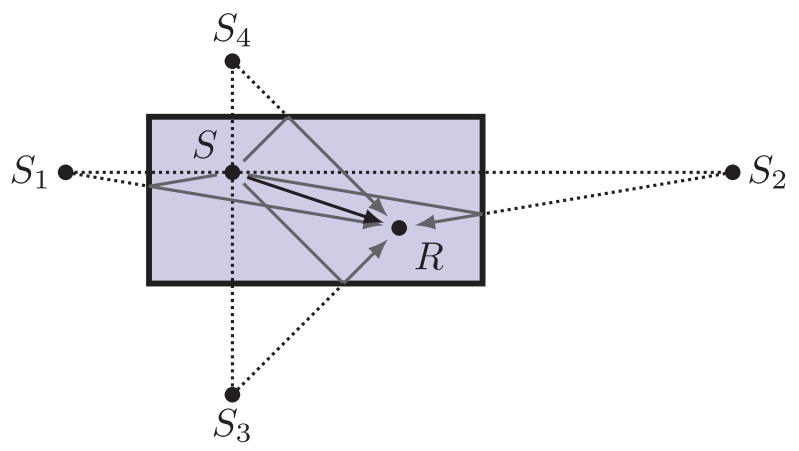
\includegraphics[width=\linewidth]{acoustics/simulator_ism2.png}
    \captionof{figure}{%
        Virtual image sources correspond to multiple sound propagation paths in the \ISM/.
        \imgsrc{\citeonly{schimmel2009fast}}
    }
    \label{fig:acoustics:simulator_ism}
}
Then, each of these image sources is itself reflected against all surfaces.
There are two main limitations of this method.
First, in a shoebox the complexity of the algorithm is cubic in the order of reflections. Therefore when an high order is required, the algorithm becomes impractical.
Second it models only the specular reflection, neglecting the diffuse sound field.
For these reasons, the image-source method is generally combined with a stochastic method in hybrid methods to model the full impulse response.

\newthought{Hybrid methods} combines the best of these two approaches.
As discussed above, the image-source method is accurate for early reflections, but slow and not accurate for longer responses.
The ray tracing method is by nature an approximation, but produces acceptable responses for diffuse fields.
And in general geometric methods fail to properly model lower frequencies and room modes.
The waveguide method models physical phenomena better than geometric methods, but is expensive at high frequencies.
All these limitations correspond to three regions in the \TFdef/ representation of the \RIR/.
As depicted in~\cref{fig:acoustics:rir_regions},

\marginpar{%
    \centering
    \footnotesize
    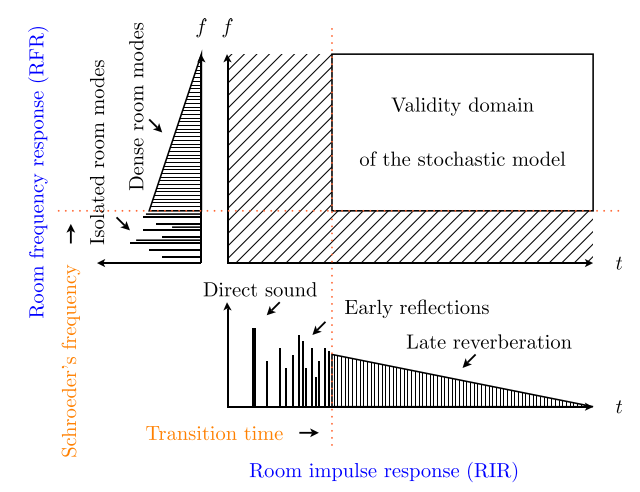
\includegraphics[width=\linewidth]{acoustics/rir_regions_stochastic.png}
    \captionof{figure}{%
    Schematic of Time-Frequency \RIR/. \imgsrc{\citeonly{badeau2019common}}.
    }
    \label{fig:acoustics:rir_regions}
}
\marginpar{%
    \centering
    \footnotesize
    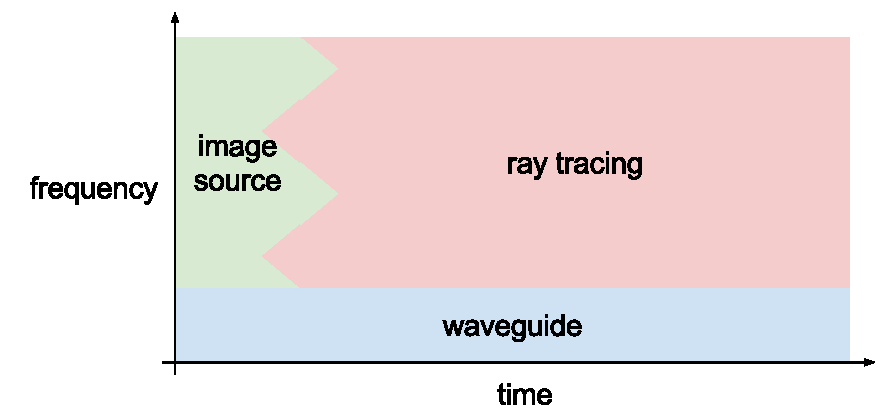
\includegraphics[width=\linewidth]{acoustics/rir_regions.pdf}
    \captionof{figure}{%
    Time-Frequency regions of \RIR/ associated to the method that better simulate them. \imgsrc{\citeonly{thomas2017wayverb}}.
    }
    \label{fig:acoustics:rir_regions}
}
\begin{itemize}
    \item in the time domain, a transition can be identified between the early \vs/ late reflection, corresponding to the validity of the deterministic \vs/ stochastic models; and
    \item in the frequency domain, between geometric \vs/ wave-based modeling.
\end{itemize}
By combining three methods, accurate broadband impulse responses can be synthesized.
However, this is possible provided that the time- and frequency-domain
\textit{crossover points} are respected and the level of each component is scaled accordingly~\citeonly{badeau2019common}.
The \textit{transition time}, or \textit{mixing time}, identifies the moment after which reflections are so frequent that they form a continuum and,
because the sound is partially absorbed by the room surfaces at every reflection,
the sound level decays exponentially over time.
This point define the cross-fade between the deterministic and the stochastic process
%\sidenote{Notice that the stochastic simulator will record both specular and diffuse reflections. Therefore, the mix between the two must be done prudently.}.
The crossover point in the frequency domain is called \textit{Schroeder's frequency}
and it split the spectrum of the \RIR/ into a region with a few isolated modes and one denser,
called respectively the \textit{resonant} and \textit{even} behaviors.
This point define the cross-fade between the geometrical and wave-based model.

Each simulator available has its own way to compute and implement this crossover points as well as mixing the results of the three methods.

\subsection{The method of images and the image source model}\label{subsec:acoustics:ism}
The \textit{Method of Images} is a mathematical tool for solving a certain class of differential equations subjected to boundary conditions.
By assuming the presence of a ``mirrored'' source, certain boundary conditions are verified facilitating the solution of the original problem.
This methods is widely used in many fields of physics, and interestingly with specific applications to Green's functions.
Its application to acoustic was originally proposed by \citeauthor{allen1979image} in \citeonly{allen1979image} and it is know as the \ISMdef/.
Now \ISM/ is probably the most used technique for deterministic \RIR/ simulation due to its conceptual simplicity and its flexibility.

The \ISM/ is based on purely specular reflection and it assumes that the sound energy travels around a scene in ``rays''.
In the appendix of \citeonly{allen1979image}, the authors also proved that this method produces a solution the Helmholtz's equation
for cuboid enclosures with rigid boundaries.

\mynewline
The image source defines the interaction of the propagating sound and the surface.
It is based on the observation that when a ray is reflected, it spawns a secondary source ``behind'' the boundary surface.
As show in~\cref{fig:acoustics:image_model}, this additional source is located on a line perpendicular to the wall, at the same distance from it as the original source, as if the original source had been “mirrored” in the surface.
In this way, each wavefront that arrives to the receiver from each reflection off the walls corresponds to the direct path received from an equivalent (or image) source.
\\The \ISM/ makes use of the following assumptions:
\begin{itemize}
    \item sound source and receiver are points in a cuboid enclosure;
    \item purely specular reflection paths between a source and a receiver;
    \item this process is simplified by assuming that sound propagates only along straight lines or rays; and
    \item rays are perfectly reflected at boundaries
\end{itemize}

% When a rigid wall is present, it represents a boundary condition to the wave equation, namely to have zero normal velocity vector.
% Assuming a lossless reflection, \ie/ $\absCoeff = 0$, a way to satisfy the boundary condition is to assume
% an additional sound source, called the \textit{image source}, placed symmetrically to the main source on the far side of the wall.
% Moreover, as discussed in~\cref{ch:acoustics:sec:reflection}, such a surface generates specular reflection.

\marginpar{%
    \centering
    \footnotesize
    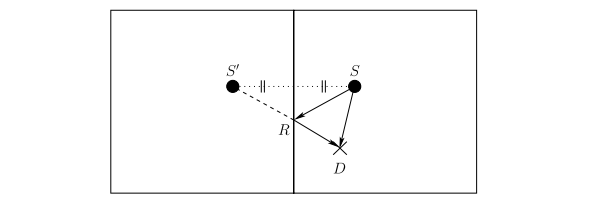
\includegraphics[width=\linewidth]{acoustics/ism_1.png}
    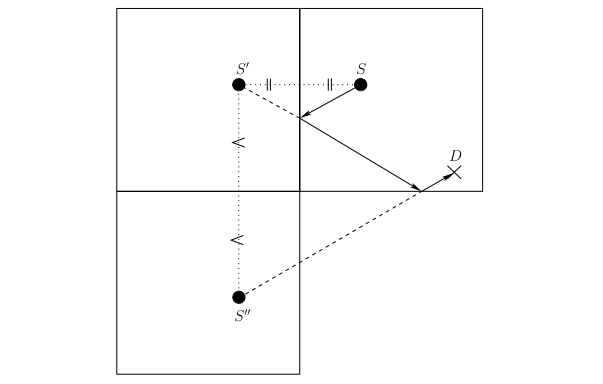
\includegraphics[width=\linewidth]{acoustics/ism_2.png}
    \captionof{figure}{%
    Path involving one reflection obtained using first-order image (top) and two reflections obtained using two images.
    It. \imgsrc{\citeonly{habets2006room}}.
    }
    \label{fig:acoustics:image_model}
}

% A sound source is located in $\positionSource$ near a reflecting wall.
% At the receiver position $\positionMicrophone$ two signals arrives: the one coming directly from $\positionSource$

% A ray which is reflected from several boundaries is represented by a “higher-order” image-source,
% which has been mirrored in each of those boundaries\citeonly{Kuttruff}. In this way, the

% All sources, original and image, emit the same impulsive source signal at the same time.
\textsc{Finally} the \RIR/ is found by summing the contribution from each (image) source, delayed and attenuated appropriately depending on their distance from the receiver.
Therefore, in the time domain, the \RIR/ associated to the source at position $\positionSource$ and the receiver at $\positionMicrophone$ reads
\begin{equation}\label{eq:acoustics:ims:time}
    \rir_{\mathtt{ISM}}(t, \positionMicrophone \mid \positionSource) =
    \sum_{\idxEch=0}^{\numEchs}
        \frac{\bar{\absCoeff}_{\idxEch}}{4 \pi \norm{\positionMicrophone - \positionSource_\idxEch}}
        \diracOf{t - \frac{\norm{\positionMicrophone - \positionSource_\idxEch}}{\speedOfSound}}
\end{equation}
where $\positionSource_\idxEch$ is the $\idxEch$-th image of the source and $\bar{\absCoeff}_{\idxEch}$
is the total frequency-independent\sidenote{Which is equivalent to consider perfectly rigid and reflective walls} damping coefficient related to the $\idxEch$-th image.
Such coefficient accounts for all the dissipation effects encountered in the reflection path, \eg/ absorption, air attention and scattering.
In the original formulation of the \ISM/, $\bar{\absCoeff}_{0} = 1$ is assumed for the direct propagation;
while for the first order images, it coincides with the frequency-independent surface absorption coefficient of the surface.
For the subsequent orders of images, the product of all the coefficient of the surfaces encounters in the reflection path is considered.

\mynewline
% The time-domain solution of the wave equation exhibits the physical essence of the echoes, that is a collection of attentions and delays.
% Although, the latter issues may be solved by using fractional delays~\citeonly{peterson1986simulating},
In order to easily incorporate frequency-dependent damping effects, the Fourier transform of~\cref{eq:acoustics:ims:time} is considered instead, where
each reflection term is appropriately scaled
\begin{equation}
    \label{eq:acoustics:ims:freq}
    \rirFreq_{\mathtt{ISM}}(f, \positionMicrophone \mid \positionSource) =
        \sum_{\idxEch=0}^{\numEchs} \frac{\absCoeff_{\idxEch}(f)}{4 \pi \norm{\positionMicrophone - \positionSource_\idxEch}}
        \exp\kparen{- \csti 2 \pi f \frac{\norm{\positionMicrophone - \positionSource_\idxEch}}{\speedOfSound}}
        ,
\end{equation}
where now the $\idxEch$-th damping coefficient $\absCoeff_{\idxEch}$ is frequency dependent.
Notice that now the damping coefficients correspond to filters, requiring~\cref{eq:acoustics:ims:time} to be written as sum of convolutions.
This have a strong implication when modeling and estimating the \RIRs/ as stream of Dirac function.
Ideally they consists of scaled Diracs with well defined time locations.
The probability that two or more Diracs arrive at the same time is then very small.
However, if we now assume that each reflection has a non-flat frequency response, filters are observed in the time domain.
Such filters have arbitrary long time-domain description and now the probability that two or more overlap is much higher.


% When simulating the discrete version of a \RIR/ on a computer, in general this distances corresponds to delays that are not on
% integer multiple of the sampling frequencies.

\mynewline
Moreover the reader should notice that the models~\eqref{eq:acoustics:ims:time, eq:acoustics:ims:freq} induce an ``order'' among reflections indexed by $\idxEch$.
Reflections are usually sorted for increasing \TOA/, $\tau_r = \norm{\positionMicrophone - \positionSource_\idxEch}/\speedOfSound$,
or decreasing amplitudes, $\bar{\absCoeff}_{\idxEch}/(4 \pi \norm{\positionMicrophone - \positionSource_\idxEch})$.
Alternatively, one can sort them according to their ``image'' generation, \eg/ direct path, first-, second-order images \etc/.
This would require an arbitrary order within the same generation, based typically on arbitrary wall sequence.
Notice that the resulting sorted sequences can differ substantially as show in~\cref{fig:acoustics:rir:ref_label}.
This translates into non trivial definition of evaluation metrics for the task of estimating echoes.

\questionpar{Can echoes be louder than the direct-path?} Yes, in certain cases reflections maybe carry energy comparable or stronger than the direct contribution.
This happens for instance when directional sources are directed towards reflectors or when multiple reflections arrive within a very short time.
Typical scenarios are when a person is presenting facing the slides projected on a wall giving the shoulders to the microphones.
When a person is very far from the microphones, the delay between each reflection is very small compare to


%%%%%%%%%%%%%%%%%%%%%%%%%%%%%%%%%%%%%%%%%%%%y
\section{Perception and some acoustic parameters}\label{ch:acoustics:sec:perception}
So far we have analyzed reverberation from a purely mathematical point of view.
However in many applications it is important to correlate physical measurements to subjective and perceptual qualities.
This will be important in order to define evaluation scenarios later in this thesis
\sidenote{
    \footnotesize
    \textbf{\textit{Cite Sacks about perception}}
}.
\subsection{The perception of the \RIR/'s elements}
It is commonly accepted that the \RIR/ components defined in~\cref{ch:acoustics:subsec:rir} play rather separate roles in the perception of sound propagation.

\newthought{The direct path} is the delayed and attenuated version of source signal itself.
It coincides with the free-field sound propagation and, as we will see in~\cref{chap:mirage}, it reveals the direction of the source.

\newthought{The early reflections and echoes} are reflections which are by nature highly correlated with to the direct sound.
They convey a sense of geometry which modifies the general perception of the sound:
\begin{description}
    \item[The precedence effect] occurs when two correlated sounds are perceived as a single auditory event~\citeonly{wallach1973precedence}.
    This happens usually when they reach the listener with a delay within $\SI{5}{\ms}$ to $\SI{40}{\ms}$.
    However, the perceived spatial location carried by the first-arriving sound suppressing the perceived location of the lagging sound.
    This allows human to accurately localize the direction of the main source, even in presence of its strong reflections.
    \item[The comb filter effect] indicates the change in timbre of the perceived sound, named \textit{coloration}.
    This happens when multiples reflections arrive with periodic patterns and some constructive or destructive interferes may arise.
    Such phenomena can be well modeled with a comb filter \citeonly{barron1971subjective}.
    \item[Apparent source width] is the audible impression of a spatially extended sound source~\citeonly{griesinger1997psychoacoustics}.
    By the presence of early reflection, the perceived energy increases, providing the impression that a source sounds larger than its true size.
    \item[Distance and depth perception] provides to the listener cues about the source location.
    While the former refers to the spatial range, the latter relates the source to the auditory scene as a whole~\citeonly{kearney2012distance}.
    A fundamental cue for distance perception is the \textit{direct-to-reverberant ratio} ($\DRR$),
    \ie/ the ratio between the direct path ratio and the remaining portion of the \RIR/.
    Regarding the depth perception, early reflections are the main responsible.
    In the context of virtual reality, correctly modeling of these quantities is essentials in order to maintain a coherent depth impression~\citeonly{kearney2012distance}.
\end{description}

\newthought{The late reverberation} in room acoustics is indicative of the size the environment and the materials within~\citeonly{valimaki2016more}.
It provides the \textit{listener envelopment}, \ie/ the degree of immersion in the sound field~\citeonly{griesinger1997psychoacoustics}.
This portion of the \RIR/ is mainly characterized by the sound diffusion, which depends on the surfaces roughness.

\subsection{Mixing time}
Perceptually, it define the instant when the reverberation cannot be distinguished from that of any other position of the listener in the room.
Analytically,  the
\begin{center}
    \textit{the mixing time is the instant that divides the early reflections from the late reverberation in a RIR},
\end{center}
% and it is represented in Equation 2.47 by $\Tmix\;[\si{\second}]$ .
Due to this, it is an important parameter also in the context of \RIRs/ synthesis as it defines cross-over point for room acoustics simulator using hybrid methods~\citeonly{savioja2015overview}\sidenote{\cfr~\cref{sec:acoustics:simulators}}.

\subsection{Reverberation time}
\marginpar{%
    \centering
    \footnotesize
    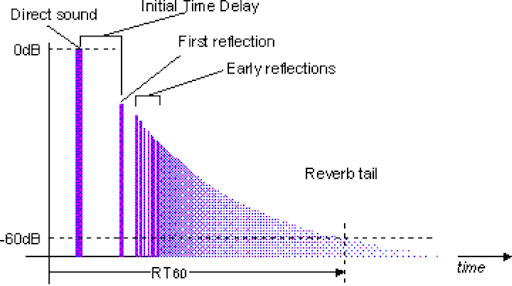
\includegraphics[width=\linewidth]{acoustics/rt60.png}
    \captionof{figure}{%
    illustration of the Reverberation Time ($\RT$) definition.
    It. \imgsrc{wikipedia}.
    }
    \label{fig:acoustics:image_model}
}
The \textit{reverberation time} measures the time that takes the sound to ``fade away'' after it ceases.
In order to quantify it, acoustics and in audio signal processing use the \textit{Reverberation Time at 60 dB}, \ie/
\begin{center}
    \textit{the $\RT$, the time after which the sound energy relatively dropped by 60 dB.}
\end{center}
It depends on the size and absorption level of the room (including obstacles), but not on the position of specific position of the source and the receiver.
Real measurements of \RIRs/ are affected by noise.
As a consequence, it is not always possible to consider a dynamic range of 60 dB,
\ie/ the energy gap between the direct path and the ground noise level.
In this case, the $\RT$ value must be approximated with other methods.
A practical approach is presented in~\cref{ap:rir:sec:rt60}.

By knowing the room geometry and the surfaces acoustics profiles,
it is possible to use the empirical \textit{Sabine's equation}:
\begin{equation}
    \RT
    \approx 0.161 \frac{V_{\text{TOT}}}{\sum_l \absCoeff_l S_l} \hspace{1em} [\si{\second}]
    ,
\end{equation}
where $V_{\text{TOT}}$ is the total volume of the room $[\si{\metre^3}]$ and $\absCoeff_l$ and $S_l$ are the
absorption coefficient and the area $[\si{\metre^2}]$  of the $l$-th surface.

\subsection{Direct-to-Reverberant ratio and the critical distance}\label{ch:acoustics:subsec:drr}
\begin{center}
    \textit{The direct-to-reverberant ratio ($\DRR$) quantifies the power of direct against indirect sound~\citeonly{zahorik2002direct}.}
\end{center}
It varies with the size and the absorption of the room, but also with the distance between the source and the receiver according to the curves
depicted in~\cref{fig:acoustics:drr}
\marginpar{%
    \centering
    \footnotesize
    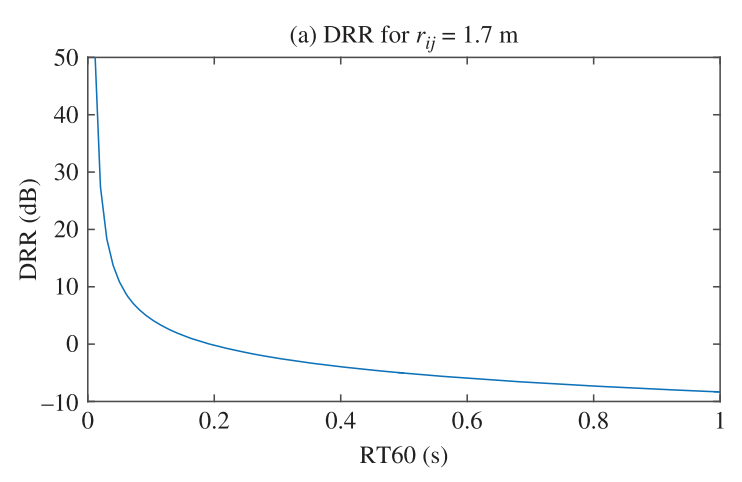
\includegraphics[width=\linewidth]{acoustics/drr_rt60.png}
    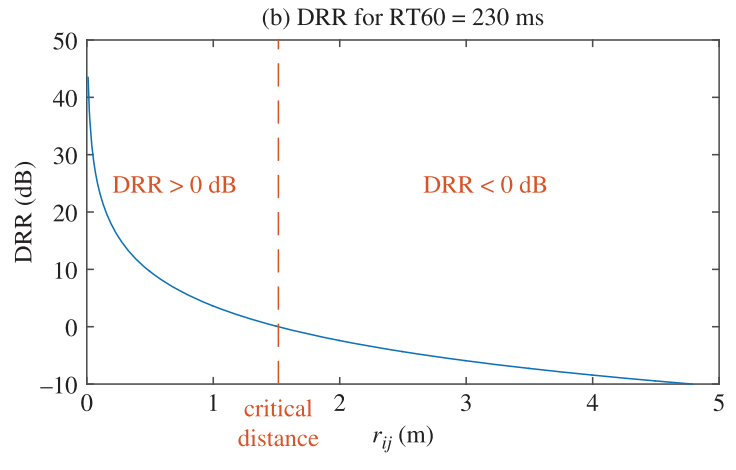
\includegraphics[width=\linewidth]{acoustics/ddr_dist.png}
    \captionof{figure}{%
        DRR as a function of the RT60 and the source distance rij based on Eyring’s formula (Gustafsson et al., 2003).
        These curves assume that there is no obstacle between the source and the microphone, so that the direct path exists.
        The room dimensions are the same as in Figure 3.1.
    }
    \label{fig:acoustics:drr}
}
% A proper analytical definition will be provided in the next chapter.
% % The $\DRR$ at the mth microphone in each microphone configuration was calculated using the method
% % \begin{equation}
% %     \DRR_\idxMic = 10 \log_{10}{\frac{
% %         \sum_{n=-\infty}^{\infty} \kparen{h^d_{ij}(n)}^2}%
% %         {\sum_{n=-\infty}^{\infty} \kparen{h^e_{ij(n)}}^2}}
% %         = 10 \log_{10}{\frac{
% %             \sum_{n=-\infty}^{\infty} \kparen{h^d_{ij}(n)}^2}%
% %             {\sum_{n=-\infty}^{\infty} \kparen{h^e_{ij}(n)}^2}}
% % \end{equation}
The distance beyond which the power of indirect sound becomes larger than that of direct sound is called the \textit{critical distance}.

These quantities represent an important parameter to assert the robustness of audio signal processing methods,
since they basically measure the validity of the free-field assumption.

% Similarly, one can define the \textit{direct-to-early ratio} ($\DER$), which is the power of direct sound divided by the remaining power in the first ??c samples (defined above),
% quantifies the modification of the power spectrum of the signal induced by early echoes.
%  It is low when the microphone and/or the source is close to an obstacle such as a table or a window, and higher otherwise.
%  The DRR and the direct-to-early ratio are not systematically reported when describing experiments in the literature,
%   yet they are as important as the RT60 to characterize multichannel mixtures
